На основе предложенного подхода к предсинтаксическому аннотированию текста на естественном языке был разработан программный модуль, выполняющий данную задачу. Разработанный программный модуль интегрирован в систему семантического анализа. Исходные коды данного программного модуля написаны на языке Java. На первой фазе разработанного подхода используется скрытая марковская модель. Скрытая марковская модель реализована на основе исходных кодов библиотеки JHMM, распространяемых под лицензией New BSD License \cite{nbsd}. Возможности данной библиотеки были расширины: реализован алгоритм обучения скрытой марковской модели с учителем, описанный в предыдущем разделе. Для этого был применен паттерн декоратор \cite{gof}.
\begin{figure}[H]
	\centering
	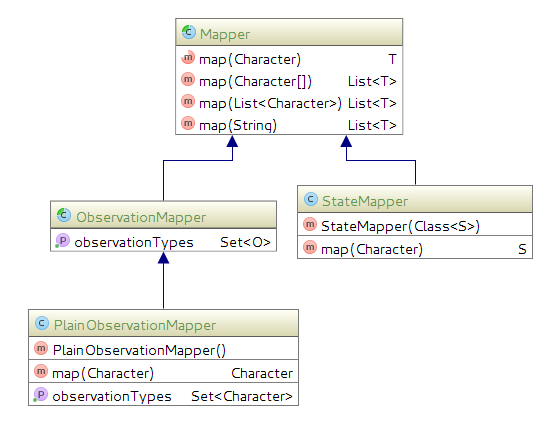
\includegraphics[scale=0.7]{img/uml_mappers.png}
	\caption{Иерархия классов, предназначенных для отображения множеств наблюдений и состояний}
\end{figure}
Для достижения возможности введения дополнительных скрытых состояний модели и определения различных множеств наблюдений был введен дополнительный уровень абстракции. На данном уровне абстракции производится отображение множества наблюдений, представленного множеством символом Unicode в другое множество наблюдений, определяемое конкретным экспериментом. 

Обучающее множество было подготовлено на основе размеченного лингвистического корпуса, составляемого в рамках проекта ``Национальный корпус русского языка'' \cite{natcorp_1, natcorp_2}. Корпус доступен для некоммерческого использования. В рамках предложенного подхода определено три скрытых состояния: внутри токена, вне токена, граница токена. Обучающее множество представляет собой множество размеченных предложений.
\begin{lstlisting}[caption={Фрагмент обучающего множества}]
 Мне жаль что тебя не застал летний ливень 
 bwb bwwb bwb bwwb bb bwwwwb bwwwwb bwwwwb
 В июльскую ночь на Балтийском заливе 
 b bwwwwwwb bwwb bb bwwwwwwwwb bwwwwb
 Не видела ты волшебства этих линий.
 bb bwwwwb bb bwwwwwwwwb bwwb bwwwb
 Волна, до которой приятно коснуться руками 
 bwwwb  bb bwwwwwb bwwwwwb bwwwwwwwb bwwwwb
 Песок, на котором рассыпаны камни 
 bwwwb  bb bwwwwwb bwwwwwwwb bwwwb
 Пейзаж, не меняющийся здесь веками.
 bwwwwb  bb bwwwwwwwwb bwwwb bwwwwb
 Мне жаль что мы снова не сядем на поезд 
 bwb bwwb bwb bb bwwwb bb bwwwb bb bwwwb
 Который пройдёт часовой этот пояс 
 bwwwwwb bwwwwwb bwwwwwb bwwb bwwb
 По стрелке которую тянет на полюс.
 bb bwwwwwb bwwwwwb bwwwb bb bwwwb
\end{lstlisting}
Каждое предложение представлено последовательностью символов алфавита естественного языка. Для каждого символа предложения поставлено в соответствие скрытое состояние. Состоянию ``граница токена'' соответствует символ ``b'', состоянию ``внутри токена'' соответствует символ ``w'', a состоянию вне токена соответствует символ `` ''. Подготовка обучающего множества заключается в преобразовании множества размеченных текстов, входящих в состав лингвистического корпуса, в множество размеченных предложений. 

В работе проведено тестирование, целью которого было составление представления об объеме обучающего множества, необходимом для достижения малой доли ошибок разметки текста. Полученное на основе лингвистического корпуса обучающее множество было разделено на две части. Первая часть использовалась алгоритмом обучения с учителем для обучения скрытой марковской модели, а вторая - для тестирования. При этом были выбраны предложения, размер которых составлял 5 - 10 слов. Количество предложений в части обучающего множества, на которой производилось обучение, изменялось от 0 до 5000 с шагом в 10 предложений. Доля ошибок расчитывалась как отношение количества предложений, в которых была допущена хоть одна ошибка разметки, к количеству предложений в тестовом множестве.
\begin{figure}[H]
	\centering
	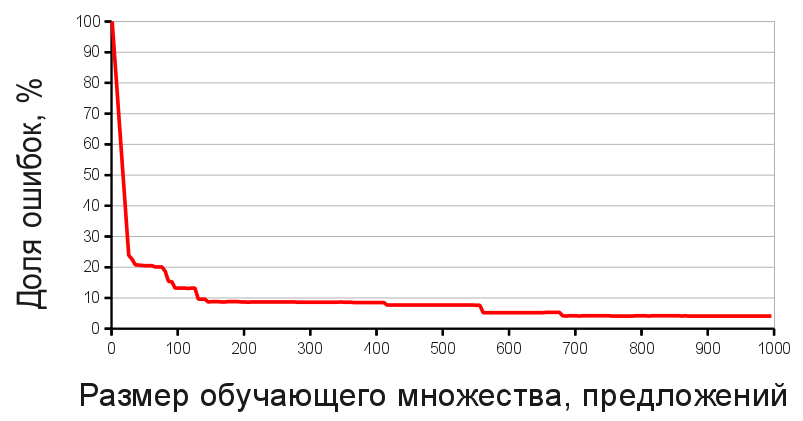
\includegraphics[scale=0.5]{img/test_chart.png}
	\caption{Доля ошибок разметки в зависимости от объема обучающего множества}
\end{figure}
В ходе тестирования было выявлено, что при достижении объема обучающего множества 690 предложений, дальнейшее увеличение объема обучающего множества не приводит к значительному изменению доли ошибок разметки.

Для реализации графового словаря была выбрана графовая база данных OrientDB \cite{web.orient}. Выбор обусловлен наличием как объектного, так и реляционного интерфеса доступа к данным, а так же наличием бинарного интерфейса поверх протокола TCP, что делает возможным обращение к данной базе данных из нативного кода без использования сторонних библиотек. Последняя возможность особенно важна ввиду того, что часть модулей системы семантического анализа написаны на языке C++.

Разработанный программный модуль предсинтаксического аннотирования текста разработан на языке Java. Сборка производится посредством системы сборки Maven \cite{maven}. Модуль доступен в виде библиотеки JAR.

Запуск предсинтаксического аннотирования осуществляется посредством вызова мотода tokenize класса, реализующего интерфейс Tokenize. Для получения экземпляра используется паттерн фабрика \cite{gof}.
\begin{lstlisting}[caption={Интерфейс модуля предсинтаксического аннотирования}]
public interface Tokenizer {

    /**
     * Выполнение предсинтаксического аннотировани текста
     *
     * @param   in  входной поток символов
     * @return      ранжированный список результатов
     */
    List<TokenizationResult> tokenize(InputStream in);

}
\end{lstlisting}
Метод tokenize возвращает ранжированный список результатов предсинтаксического аннотирования. Результат аннотирования реализует интерфейс TokenizationResult, позволяющий получить список найденных токенов и значение критерия ранжирования, соответствующее данному результату.
\begin{lstlisting}[caption={Интерфейс результата аннотирования}]
public interface TokenizationResult {

    /**
     * Получение значения критерия ранжирования 
     * для данного результата
     */
    double getK();

    /**
     * Получение списка токенов
     */
    List<Token> getTokens();

}
\end{lstlisting}
Токен имеет интерфейс, позволяющий получить исходную последовательность символов, соответствующую найденному токену, и последовательность символов с внесенными корректировками. Также имеется возможность получить список установленных аттрибутов и ссылку на узел графового словаря, если найденный токен является словоформой.
\begin{lstlisting}[caption={Интерфейс токена}]
public interface Token {

    /**
     * Исходная последовательность символов,
     * соответствующая данному токену
     */
    char[] getSeq();

    /**
     * Последовательность символов с применением корректировок,
     * соответствующая данному токену
     */
    char[] getModifiedSeq();

    /**
     * Ссылка на узел графового словаря
     */
    Long getDictNodeId();

    /**
     * Список установленных атрибутов
     */
    List<Attribute> getAttributes();

}
\end{lstlisting}